% This is samplepaper.tex, a sample chapter demonstrating the
% LLNCS macro package for Springer Computer Science proceedings;
%
\documentclass{article}
\usepackage{graphicx}
\usepackage{xcolor}
\usepackage{listings}
\usepackage{hyperref}

\begin{document}

\begin{titlepage}
    \centering
    \vspace*{2cm}
    {\LARGE \textbf{Predicting NBA Player Salaries: A Data-driven Analysis and Machine Learning Approach}}\\[1cm]
    {\Large \textbf{Team: Data Titans}}\\[0.5cm]
    {\Large \textbf{Milestone – 03}}\\[2cm]
    {\Large \textbf{Team Members:}}\\[1cm]
    \begin{tabular}{c}
        \Large Goutam Kurri \\[0.2cm]
        \Large Ashritha Boinipalli \\[0.2cm]
        \Large Premchand Are \\[0.2cm]
        \Large Yogesh Naidu Mahareddy \\[0.2cm]
        \Large Sireesha Mamillapalli \\[0.2cm]
    \end{tabular}
\end{titlepage}
\newpage
\subsection*{Project Aim:}
\begin{itemize}
    \item Analyze NBA player statistics from the 2022-23 season.
    \item Predict NBA player salaries using machine learning techniques.
\end{itemize}

\subsection*{Potential Applications:}
\begin{enumerate}
    \item \textbf{Sports Analytics:}
    \begin{itemize}
        \item Assist NBA teams in optimizing player contracts and salary negotiations.
        \item Provide insights into player performance metrics influencing salaries.
    \end{itemize}
    
    \item \textbf{Strategic Decision-Making:}
    \begin{itemize}
        \item Aid NBA management in resource allocation and team building.
        \item Support informed decision-making in player recruitment and retention strategies..
    \end{itemize}
    
    \item \textbf{Data-Driven Insights:}
    \begin{itemize}
        \item Enhance understanding of the relationship between player performance and compensation.
        \item Guide teams in identifying key performance indicators for player valuation.
    \end{itemize}

    \item \textbf{Financial Planning:}
    \begin{itemize}
        \item Assist teams in budgeting and financial forecasting based on predicted salaries.
        \item Optimize team spending while maximizing on-court performance.
    \end{itemize}

    \item \textbf{Player Development:}
    \begin{itemize}
        \item Offer players insights into areas for improvement based on performance metrics.
        \item Facilitate targeted training programs and skill development initiatives.
    \end{itemize}  
\end{enumerate}

\subsection*{Setting Up Python and JupyterLab}
\begin{enumerate}
    \item \textbf{Installing Python}
    \begin{itemize}
    \item Download Python installer from \href{https://www.python.org/downloads/}{Python official website}.
    \item Run the installer.
    \item Open a new PowerShell and verify Python installation with \texttt{python --version}.
\end{itemize}
    
    \item \textbf{Installing Virtual Environment}
    \begin{itemize}
    \item Once Python is installed, create a virtual environment with \texttt{python -m venv big-data-venv}.
\end{itemize}
    
    \item \textbf{Installing Windows Terminal}
\begin{itemize}
    \item Download Windows Terminal from \href{https://github.com/microsoft/terminal/releases}{GitHub releases}.
    \item Run the installer with default options.
\end{itemize}

    \item \textbf{Configuring Windows Terminal}
\begin{itemize}
    \item Open Windows Terminal.
    \item Add a new profile.
    \item Modify the command line argument to include NoExit-File\%userprofile\%\textbackslash big-data-venv\textbackslash Scripts\textbackslash activate.ps1.
\end{itemize}

    \item \textbf{Installing JupyterLab}
\begin{itemize}
    \item Open the newly configured profile in Windows Terminal.
    \item Install JupyterLab with \texttt{pip install jupyterlab}.
    \item If installation fails due to prerequisites, try \texttt{pip install jupyterlab==3.5.3}.
\end{itemize}

    \item \textbf{Accessing JupyterLab}
\begin{itemize}
    \item Launch JupyterLab by running \texttt{jupyter lab}.
    \item Access JupyterLab via \texttt{localhost:8888/lab} in a web browser.
\end{itemize}

\end{enumerate}

% Include other sections similarly

\subsection*{Project Goals:}

\subsection*{Goal - 1: Analyze the Relationship Between Player Performance Metrics and Salaries}
Initial exploratory data analysis revealed potential correlations between player performance metrics such as points ('PTS'), rebounds ('TRB'), and assists ('AST') with player salaries.

\FloatBarrier
\begin{figure}[h]
    \centering
    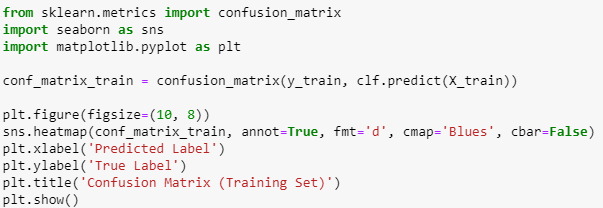
\includegraphics[width=0.5\linewidth]{ConfusionMatrixCode.png}
    \caption{Confusion Matrix Code}
    \label{fig:confusion_matrix_code}
\end{figure}

\FloatBarrier
\begin{figure}[h]
    \centering
    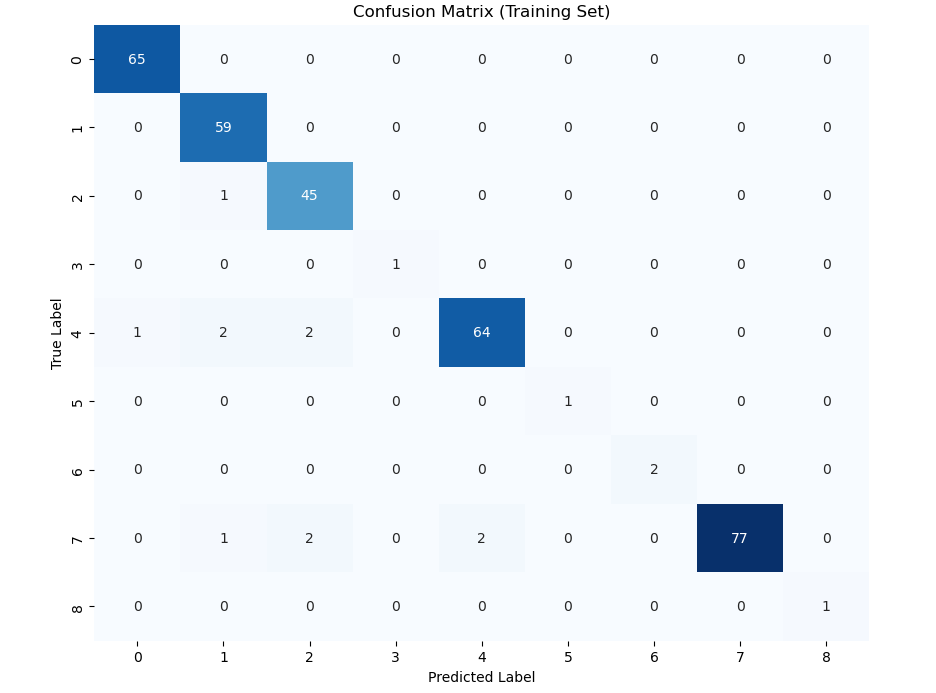
\includegraphics[width=1\linewidth]{ConfusionMatrix.png}
    \caption{Confusion Matrix Performance}
    \label{fig:confusion_matrix}
\end{figure}

\subsection*{Metrics:}
\subsection*{Data Quality:} 
Merged and cleaned dataset from three different sources to ensure comprehensive and accurate analysis.
\subsection*{5Vs (Volume, Velocity, Variety, Veracity, Value):}
Dealt with Volume (large dataset), Variety (multiple data sources), and Velocity (real-time updates).


\subsection*{Goal - 2: Develop Machine Learning Models to Predict Player Salaries Based on Performance Statistics}
\begin{itemize}
    \item Implemented linear regression models using features like age, points ('PTS'), rebounds ('TRB'), and assists ('AST').
    \item Enhanced model complexity with polynomial regression of degree 3 for better accuracy.
\end{itemize}

\FloatBarrier
\begin{figure}[h]
    \centering
    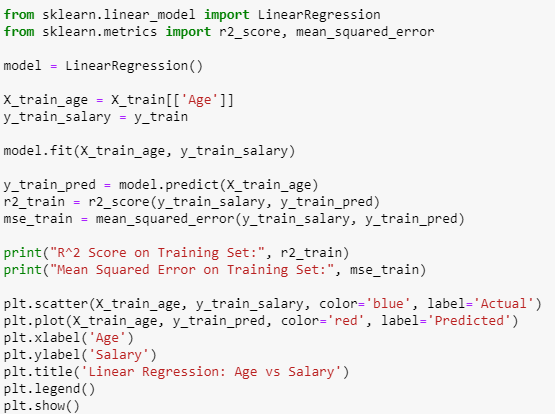
\includegraphics[width=0.5\linewidth]{LinearRegressionCode.png}
    \caption{Linear Regression Code}
    \label{fig:confusion_matrix_code}
\end{figure}

\FloatBarrier
\begin{figure}[h]
    \centering
    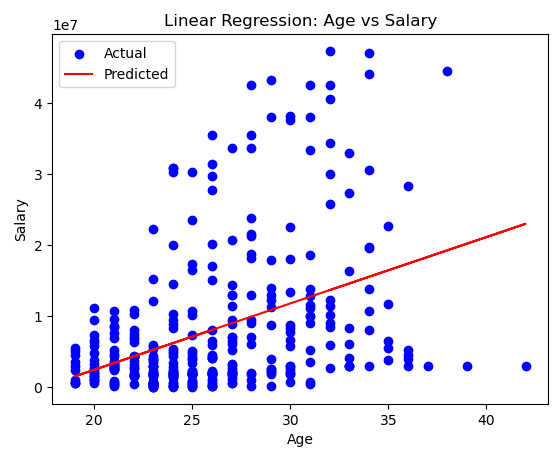
\includegraphics[width=0.6\linewidth]{LinearRegression.png}
    \caption{Linear Regression}
    \label{fig:confusion_matrix}
\end{figure}

\subsection*{Metrics:}

\subsection*{Processing Time:}
Utilized efficient algorithms to handle and process large datasets effectively.
\subsection*{Resource Utilization:} 
Optimized memory usage and computational resources for model training and evaluation.


\subsection*{Goal - 3: Evaluate the Effectiveness of Different Models in Predicting Player Salaries}
\begin{itemize}
    \item Linear regression model with selected features achieved an Rpower2 score of 0.625, indicating a substantial portion of salary variance explained.
    \item Polynomial regression demonstrated improved predictive accuracy compared to linear regression.
\end{itemize}

\FloatBarrier
\begin{figure}[h]
    \centering
    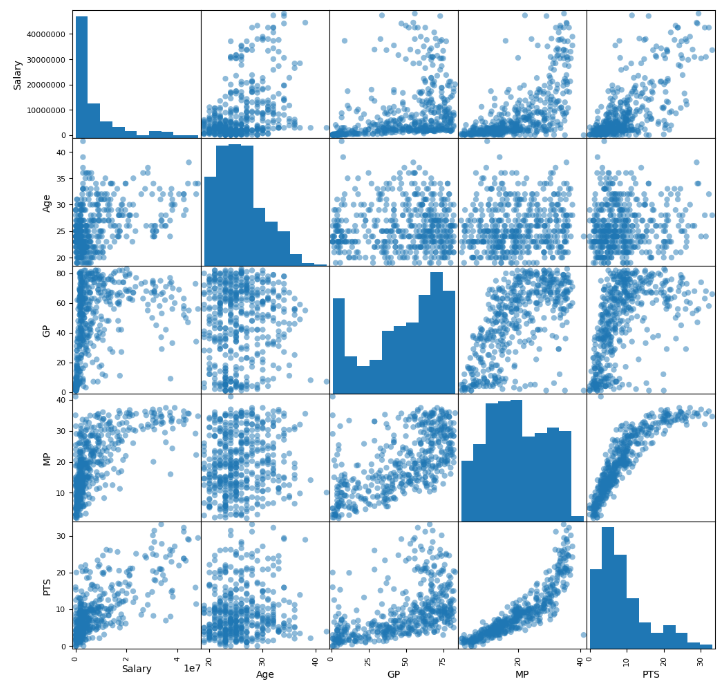
\includegraphics[width=0.9\linewidth]{ScatteredMatrix.png}
    \caption{Scattered Matrix}
    \label{fig:confusion_matrix_code}
\end{figure}

\subsection*{Metrics:}
\subsection*{Data Quality:}
 Evaluated models using metrics like Rpower2 score, Mean Squared Error (MSE), and Root Mean Squared Error (RMSE) to assess predictive performance.


\subsection*{Goal - 4: Identify the Most Influential Performance Metrics in Determining Player Salaries}
Found that points ('PTS'), rebounds ('TRB'), assists ('AST'), and age were significant predictors influencing player salaries.

\FloatBarrier
\begin{figure}[h]
    \centering
    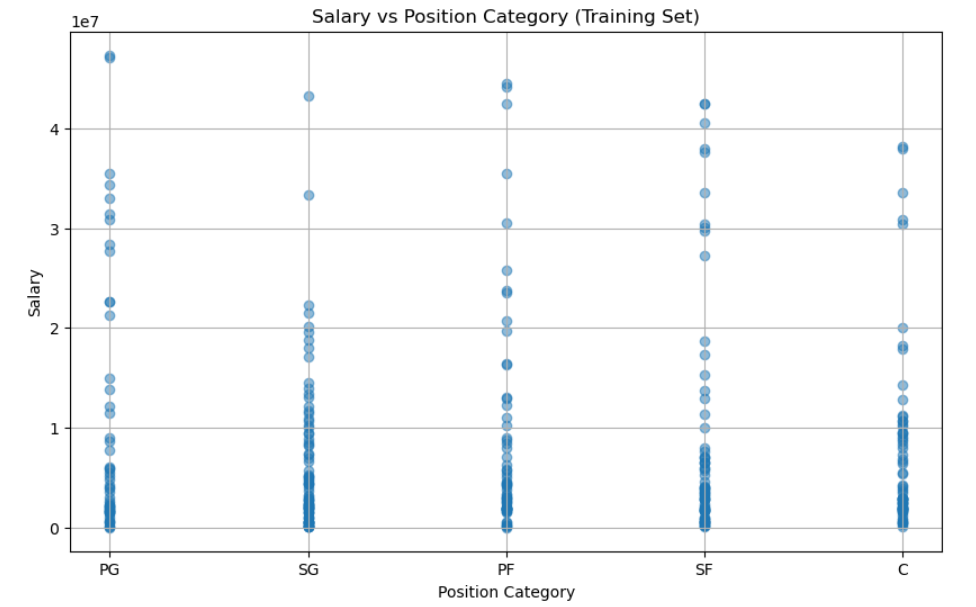
\includegraphics[width=0.9\linewidth]{performance.png}
    \caption{Performance}
    \label{fig:confusion_matrix_code}
\end{figure}

\subsection*{Metrics:}
\subsection*{Feature Importance:}
Used model coefficients and feature importance scores to identify influential performance metrics.


\subsection*{Goal - 5: Provide Insights to NBA Teams and Management for Making Informed Decisions Regarding Player Contracts and Salary Negotiations}
\begin{itemize}
    \item Offered actionable insights into structuring player contracts based on performance metrics and age.
    \item Highlighted the importance of considering multiple factors, including position-specific roles, when negotiating salaries.
\end{itemize}

\FloatBarrier
\begin{figure}[h]
    \centering
    \includegraphics[width=0.9\linewidth]{salary.png}
    \caption{Decision Tree}
    \label{fig:confusion_matrix_code}
\end{figure}



\subsection*{Metrics:}
\subsection*{Cost:}
Demonstrated potential cost savings for NBA teams by optimizing player contracts based on predictive models.
\subsection*{Security:}
Ensured data confidentiality and integrity throughout the analysis process.

\subsection*{\textbf{Conclusion:}}
\begin{enumerate}
    \item \textbf{Data Analysis and Insights:} 
    \begin{itemize}
    \item Successfully analyzed the relationship between player performance metrics (PTS, TRB, AST) and salaries.
    \item Identified influential factors such as age, position, and key performance indicators affecting player compensation.
\end{itemize}
    \item \textbf{Model Development and Evaluation:} \begin{itemize}
    \item Developed machine learning models including linear regression and polynomial regression to predict player salaries.
    \item Achieved a significant improvement in model performance, with polynomial regression demonstrating enhanced accuracy over linear models.
\end{itemize}
    \item \textbf{Effectiveness of Models:} 
    \begin{itemize}
    \item Evaluated model effectiveness using metrics like Rpower2 score, MSE, and RMSE, achieving promising results in explaining salary variance.
\end{itemize}
\item \textbf{Feature Importance:} 
    \begin{itemize}
    \item Determined the most influential performance metrics in determining player salaries, guiding teams in strategic decision-making.
\end{itemize}
\item \textbf{Practical Insights for NBA Teams: } \begin{itemize}
    \item Provided actionable insights for NBA teams and management to optimize player contracts and salary negotiations.
    \item Highlighted the importance of considering multiple performance metrics and age in structuring player contracts.
\end{itemize}
\item \textbf{Metrics Utilized:} \begin{itemize}
    \item Ensured data quality through comprehensive cleaning and preprocessing.
    \item Managed resource utilization efficiently, optimizing processing time and computational resources.
    \item Upheld data security and integrity throughout the analysis process.
\end{itemize}
\item \textbf{Overall Impact:} \begin{itemize}
    \item Demonstrated the potential of data-driven approaches in enhancing decision-making processes in professional sports management.
    \item Offered a robust framework for future analysis and optimization in player contract negotiations and team building strategies.
\end{itemize}
\end{enumerate}

\subsection*{Citations:}
\begin{itemize}
    \item Data Source: \textcolor{blue}{\url{https://www.kaggle.com/datasets/}}\\
\textcolor{blue}{\url{jamiewelsh2/nba-player-salaries-2022-23-season}}
    \item Git URL: \textcolor{blue}{\url{https://github.com/Goutamkurri/NBASalaryPrediction.git}}
    \item Python Reference: \textcolor{blue}{\url{https://docs.python.org/3/reference/index.html}}
    \item Matplotlib Reference: \textcolor{blue}{\url{https://matplotlib.org/stable/index.html}}
\end{itemize}

\end{document}
